\title{Matrix Multiplication}
\subtitle{\SubTitleName}
\institute[]{\Course}
\author{\Instructor}
\maketitle

\tikzstyle{startstop} =[trapezium, trapezium left angle=70, trapezium right angle=110, minimum width=1cm, minimum height=1cm, text centered, fill=Teal!30]

\tikzstyle{io} = [trapezium, trapezium left angle=70, trapezium right angle=110, minimum width=1cm, minimum height=1cm, text centered, fill=DarkRed!30]

\tikzstyle{process} = [trapezium, trapezium left angle=70, trapezium right angle=110, minimum width=1cm, minimum height=1cm, text centered, fill=Gold!60]

\tikzstyle{arrow} = [thick,->,>=stealth]

\frame{\frametitle{Motivation}
    \pause
    Application: multiple linear transforms. 
    \pause 
    
    \Emph{Objectives}\\
    
    \LearningObjectiveStatement
    
    \begin{itemize}

        \item multiply matrices using two different methods

        % \item determine whether the multiplication of two matrices is defined

        % \item apply the properties of matrix multiplication to analyze matrix equations
        
        % \item apply matrix algebra and the zero and identity matrices to solve and analyze matrix equations

    \end{itemize}
}


% First slide - Definition (keeping the original)
% \frame{\frametitle{Matrix Multiplication}
% \vspace{-12pt}
% \begin{center}\begin{tikzpicture} \node [mybox](box){\begin{minipage}{0.95\textwidth}
%     Let $ A $ be an $ m \times n $ matrix, and $ B$ be an $ n \times p$ matrix. \onslide<2->{ The product  $ A B  $ is an $ m \times p$ matrix,} \onslide<3->{equal to} \onslide<4->{$$ A B = A 
%     \begin{pmatrix}
%     \vec b_1 & \cdots & \vec b_p
%     \end{pmatrix} = 
%     \begin{pmatrix}
%     A \vec b_1 & \cdots & A \vec b_p
%     \end{pmatrix}
%     $$ }
%     \end{minipage}};
%     \node[fancytitle, right=10pt] at (box.north west) {Definition};
%     \end{tikzpicture}\end{center}
% }

\frame{\frametitle{Definition: Matrix Multiplication}

\vspace{-12pt}
\begin{center}\begin{tikzpicture} \node [mybox](box){\begin{minipage}{0.95\textwidth}

    Let $ A $ be an $ m \times n $ matrix, and $ B$ be an $ n \times p$ matrix. \onslide<2->{ The product  $ A B  $ is an $ m \times p$ matrix,} \onslide<3->{equal to} \onslide<4->{$$ A B = A 
    \begin{pmatrix}
    \vec b_1 & \cdots & \vec b_p
    \end{pmatrix} = 
    \begin{pmatrix}
    A \vec b_1 & \cdots & A \vec b_p
    \end{pmatrix}
    $$ }
    \end{minipage}};
    \node[fancytitle, right=10pt] at (box.north west) {Definition};
    \end{tikzpicture}\end{center}

    \onslide<5->{
    \Emph{Example} \\
    
    Compute the following product. 
    
    \begin{equation*}
    C = AB = 
    \spalignmat{2 0;1 1}\spalignmat{2 0 0;3 4 0}
    \end{equation*}
    }

}







% % New slide - Visual introduction to the example
% \frame{\frametitle{Matrix Multiplication Example}
%     Let's multiply these matrices step by step:
%     \vspace{8pt}
    
%     \onslide<1->{
%     \begin{equation*}
%     C = A B = 
%     \begin{pmatrix} 2 & 0 \\ 1 & 1 \end{pmatrix}
%     \begin{pmatrix} 2 & 0 & 0 \\ 3 & 4 & 0 \end{pmatrix}
%     \end{equation*}
%     }
    
%     \onslide<2->{
%     \begin{itemize}
%         \item The result $C$ will be a $2 \times 3$ matrix
%         \item We'll compute each entry using the row-column method
%         \item Highlighted rows and columns will show which numbers we're using
%     \end{itemize}
%     }
% }

% % Computing first entry with highlighting
% \frame{\frametitle{Computing $c_{11}$ (First Entry)}
%     \begin{center}
%     $\begin{pmatrix} \rowcolor{blue!10} 2 & 0 \\ 1 & 1 \end{pmatrix}$
%     $\begin{pmatrix} \multicolumn{1}{>{\columncolor{green!10}}c}{2} & 0 & 0 \\ \multicolumn{1}{>{\columncolor{green!10}}c}{3} & 4 & 0 \end{pmatrix}$
    
%     \vspace{8pt}
%     $c_{11} = (2)(2) + (0)(3) = 4$
    
%     \vspace{8pt}
%     Result so far:
%     $C = \begin{pmatrix} \mathbf{4} & ? & ? \\ ? & ? & ? \end{pmatrix}$
%     \end{center}
% }

% % Computing second entry
% \frame{\frametitle{Computing $c_{12}$ (Second Entry)}
%     \begin{center}
%     $\begin{pmatrix} \rowcolor{blue!10} 2 & 0 \\ 1 & 1 \end{pmatrix}$
%     $\begin{pmatrix} 2 & \multicolumn{1}{>{\columncolor{green!10}}c}{0} & 0 \\ 3 & \multicolumn{1}{>{\columncolor{green!10}}c}{4} & 0 \end{pmatrix}$
    
%     \vspace{8pt}
%     $c_{12} = (2)(0) + (0)(4) = 0$
    
%     \vspace{8pt}
%     Result so far:
%     $C = \begin{pmatrix} 4 & \mathbf{0} & ? \\ ? & ? & ? \end{pmatrix}$
%     \end{center}
% }

% % Computing third entry
% \frame{\frametitle{Computing $c_{21}$ (Third Entry)}
%     \begin{center}
%     $\begin{pmatrix} 2 & 0 \\ \rowcolor{blue!10} 1 & 1 \end{pmatrix}$
%     $\begin{pmatrix} \multicolumn{1}{>{\columncolor{green!10}}c}{2} & 0 & 0 \\ \multicolumn{1}{>{\columncolor{green!10}}c}{3} & 4 & 0 \end{pmatrix}$
    
%     \vspace{8pt}
%     $c_{21} = (1)(2) + (1)(3) = 5$
    
%     \vspace{8pt}
%     Result so far:
%     $C = \begin{pmatrix} 4 & 0 & ? \\ \mathbf{5} & ? & ? \end{pmatrix}$
%     \end{center}
% }

% % Computing fourth entry
% \frame{\frametitle{Computing $c_{22}$ (Fourth Entry)}
%     \begin{center}
%     $\begin{pmatrix} 2 & 0 \\ \rowcolor{blue!10} 1 & 1 \end{pmatrix}$
%     $\begin{pmatrix} 2 & \multicolumn{1}{>{\columncolor{green!10}}c}{0} & 0 \\ 3 & \multicolumn{1}{>{\columncolor{green!10}}c}{4} & 0 \end{pmatrix}$
    
%     \vspace{8pt}
%     $c_{22} = (1)(0) + (1)(4) = 4$
    
%     \vspace{8pt}
%     Result so far:
%     $C = \begin{pmatrix} 4 & 0 & ? \\ 5 & \mathbf{4} & ? \end{pmatrix}$
%     \end{center}
% }

% % Computing fifth and sixth entries
% \frame{\frametitle{Computing Final Entries ($c_{13}$ and $c_{23}$)}
%     \begin{center}
%     For $c_{13}$:
%     $\begin{pmatrix} \rowcolor{blue!10} 2 & 0 \\ 1 & 1 \end{pmatrix}$
%     $\begin{pmatrix} 2 & 0 & \multicolumn{1}{>{\columncolor{green!10}}c}{0} \\ 3 & 4 & \multicolumn{1}{>{\columncolor{green!10}}c}{0} \end{pmatrix}$
    
%     $c_{13} = (2)(0) + (0)(0) = 0$
    
%     \vspace{8pt}
%     For $c_{23}$:
%     $\begin{pmatrix} 2 & 0 \\ \rowcolor{blue!10} 1 & 1 \end{pmatrix}$
%     $\begin{pmatrix} 2 & 0 & \multicolumn{1}{>{\columncolor{green!10}}c}{0} \\ 3 & 4 & \multicolumn{1}{>{\columncolor{green!10}}c}{0} \end{pmatrix}$
    
%     $c_{23} = (1)(0) + (1)(0) = 0$
%     \end{center}
% }

% % Complete result
% \frame{\frametitle{Complete Matrix Multiplication}
%     \begin{center}
%     Final result:
    
%     \vspace{8pt}
%     \onslide<1->{
%     $C = AB = \begin{pmatrix} 4 & 0 & 0 \\ 5 & 4 & 0 \end{pmatrix}$
%     }
    
%     \vspace{12pt}
%     \onslide<2->{
%     \begin{tikzpicture} \node [mybox](box){\begin{minipage}{0.85\textwidth}
%     Each entry $c_{ij}$ is computed by:
%     \begin{itemize}
%         \item Taking row $i$ from matrix $A$ (highlighted in blue)
%         \item Taking column $j$ from matrix $B$ (highlighted in green)
%         \item Computing their dot product for entry $(i,j)$ in matrix $C$
%     \end{itemize}
%     \end{minipage}};
%     \node[fancytitle, right=10pt] at (box.north west) {Key Insight};
%     \end{tikzpicture}
%     }
%     \end{center}
% }

% % Final summary slide
% \frame{\frametitle{Summary}
%     \SummaryLine \vspace{4pt}
    
%     \begin{itemize}\setlength{\itemsep}{8pt}
%         \item Each entry in the product matrix comes from one row of $A$ and one column of $B$
%         \item The dot product of the row and column gives the entry value
%         \item The dimensions must match: $(m \times n)(n \times p) = (m \times p)$
%         \item The order of multiplication matters - matrix multiplication is not commutative
%     \end{itemize}
    
%     \vspace{8pt}
%     \begin{center}
%     \colorbox{red!2}{Practice: Try computing $BA$ (if possible) to see why order matters!}
%     \end{center}
% }









% \frame{\frametitle{Summary}

%     \SummaryLine \vspace{4pt}
    
%     \begin{itemize}\setlength{\itemsep}{8pt}
%         \item multiplying matrices by multiplying the first matrix with each column of the second matrix
%         \item multiplying matrices with the \textbf{row column method}
%     \end{itemize}
%     \vspace{4pt}
%     \pause
%     There are several ways of multiplying matrices. This video introduced two methods. 
% }

% \frame{
% }





\title{Properties of Matrix Multiplication}
\subtitle{\SubTitleName}
\institute[]{\Course}
\author{\Instructor}
\maketitle


\tikzstyle{startstop} =[trapezium, trapezium left angle=70, trapezium right angle=110, minimum width=1cm, minimum height=1cm, text centered, fill=Teal!30]

\tikzstyle{io} = [trapezium, trapezium left angle=70, trapezium right angle=110, minimum width=1cm, minimum height=1cm, text centered, fill=DarkRed!30]

\tikzstyle{process} = [trapezium, trapezium left angle=70, trapezium right angle=110, minimum width=1cm, minimum height=1cm, text centered, fill=Gold!60]

\tikzstyle{arrow} = [thick,->,>=stealth]

\frame{\frametitle{Topics and Objectives}
    \Emph{Topics} \\
    \TopicStatement
    \begin{itemize}
    
        \item properties of matrix multiplication 
        
    \end{itemize}
    
    \vspace{0.5cm}
    
    \Emph{Objectives}\\
    
    \LearningObjectiveStatement
    
    \begin{itemize}

        \item determine whether the multiplication of two matrices is defined

        \item apply the properties of matrix multiplication to analyze matrix equations
        
        % \item apply matrix algebra and the zero and identity matrices to solve and analyze matrix equations

    \end{itemize}


}

\frame{\frametitle{Matrix Dimensions and Matrix Multiplication}

    Note: the dimensions of $A$ and $B$ determine whether $AB$ is defined, and what its dimensions will be.
    
    \begin{center}
        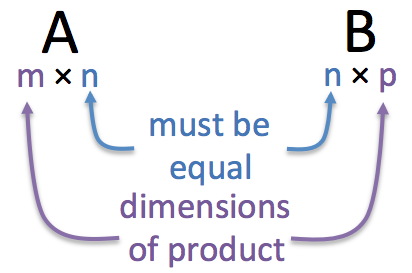
\includegraphics[width=0.3\textwidth]{Chapter2/images/matrix_multi2} 
    \end{center}

}

\frame{\frametitle{Properties of Matrix Multiplication} 

    \onslide<2->{Let $ A, B, C$ be matrices of the sizes needed for the matrix multiplication to be defined, and $ A $ is a $ m \times n$ matrix.}
    
    \begin{enumerate}
        \item<3-> (Associative)  $(AB)C= A (BC)$ 
        \item<4-> (Left Distributive)  $A (B+C) = AB + AC $ 
        \item<4-> (Right Distributive) $(A + B)C = AC + BC $ 
        \item<5-> (Identity for matrix multiplication)  $ I _{m} A = A I _{n}$ 
    \end{enumerate}

    \onslide<6->{
    \Emph{\color{Teal}Warnings:}  
    }
    \begin{enumerate}
        \item<7->  (non-commutative) In general, $ AB \neq BA $. \pause  
        \item<8->  (non-cancellation) $ AB = A C $ does not mean $ B=C$. \pause 
        \item<9->  (Zero divisors) $ AB = 0$ does not mean that either $ A=0$ or $ B=0$.  
    \end{enumerate}

}

\frame{\frametitle{Examples}
    Suppose $A = \spalignmat{1 0; 0 0}$.
    \begin{enumerate}
        \item Give an example of a $2\times2$ matrix that does not commute with $A$. 
        \item Construct any non-zero matrices $B$ and $C$ so that $B\ne C$ but $AB=AC$.
    \end{enumerate}
    
}


\frame{\frametitle{The Associative Property} 

    If $C = \vec x$, then the associative property is: $(AB)\vec x = A (B \vec x)$. Schematically: 
    
    \vspace{18pt}
    
    \begin{tikzpicture}[node distance=2cm]

        \node(x)  [startstop] {$\vec x$};
        \node(bx) [io, below of=x] {$B\vec x$};
        \node(abx)[process, right of=x,xshift=4cm]{$AB\vec x$};
        
        \draw [arrow] (x) -- node[anchor=east] {\small Multiplication by $B$} (bx);
        \draw [arrow] (bx) -- node[anchor=north,xshift=1.2cm] {\small Multiplication by $A$} (abx);
        \draw [arrow] (x) --node[anchor=south] {\small  \ \ \ Multiplication by $AB$} (abx);
        
    \end{tikzpicture}

    \vspace{4pt}

    The matrix product $ AB\vec x$ can be obtained by either: multiplying by matrix $AB$, or by multiplying by $B$ then by $A$. This means that matrix multiplication corresponds to \Emph{composition of the linear transformations}.
}

% 


% \begin{frame}
% \frametitle{Additional Examples}

%     True or false:

%     \begin{enumerate}
%         \item For any $I_n$ and any $A \in \R^{n\times n}$, $(I_n + A)(I_n - A) = I_n - A^2$. \\[3cm]
%         \item For any $A$ and $B$ in $\R^{n\times n}$, $(A+B)^2 = A^2 + B^2 + 2AB$. 
%     \end{enumerate}

% \end{frame}

\frame{\frametitle{Summary}

    \SummaryLine \vspace{4pt}
    \pause 
    \begin{itemize}\setlength{\itemsep}{8pt}
        \item using matrix dimensions to determine whether a matrix product is defined and what the dimensions of the product will be\pause 
        \item applying properties of matrix algebra to analyze matrix equations
    \end{itemize}
    \vspace{4pt}
    
}

\frame{
}

\frame{
}
